\chapter{Ontology Based Knowledge Management For Multimedia Indexing}


\section{Introduction}

A number of diverse approaches for semantic multimedia content analysis have been proposed addressing the discovery of features ranging from low-level features \cite{Brunelli1999,Antani2002,Kang2003,Smith2003} (color, histograms, \dots{}) to high-level ones \cite{Snoek2006, Lew2006,Spyrou2008} (semantic objects and concepts). However, these earlier approaches failed to reduce the semantic gap and were not able to deliver an efficient semantic interpretation \cite{Snoek2010,Over2013}. Under such context, exploring further semantics within a multimedia content is a prerequisite and a major challenge.

Towards this goal, further semantic information, other than low-level and concepts one, are gathered from a multimedia content in order to enhance semantic interpretation capabilities. Motived by a kindred vision of human perception, yet targeting automated analysis of a multimedia content, the multimedia retrieval community addressed more attention to content contexts \cite{Mylonas2009, Nguyen2010, Elleuch2011,PerpetualCoutinho2012} and concepts co-occurency \cite{Naphade2006,Vallet2007,
Mylonas2008,Mylonas2009,Elleuch2011,Paliouras2011}. While a concepts co-occureny relies on potential relationship that can exists between two objects in a content, the context could precises a set of concepts that can exist in that content. For instance, \emph{``Beach''} and \emph{``Sand''} can be considered as two co-occurred concepts since the existence of the \emph{``Beach''} led to found the concept \emph{``Sand''}. Also, in the context of \emph{``Car Racing''}, concepts \emph{``Car''}, \emph{``Racetrack''}, \emph{``Crowd''}, \dots{} could co-exist in the same content. 

Aspiring to reconcile and exploit the semantic assets provided by the two proposals, namely the concepts co-occurnece and contexts, a number of initiatives have investigated the engineering of knowledge-based approaches for multimedia retrieval. Yet, ontologies (as a knowledge database) are powerful tools to design concepts/contexts and their interrelationships. In general, ontology-based approaches consists in defining a knowledge conceptualization and a reasoning process in order to handle and enhance a semantic interpretation. An immediate effect of such efforts is the alleviation of the semantic barriers and many promising works raised \cite{Kannan2012}. However, these recent approaches still facing some issues related to the construction of the ontology and its content. 

At fisrt, ontology contents used for information retrieval systems are generally outlined  manually or for specific field/domain 
like medicine \cite{Rozilawatibinti2011}, Athletics \cite{Paliouras2011}, \dots. The manual design of an ontology is a high cost process \cite{Song2009}. In order to tackle this problem, an automated method for ontology population should be addressed.

Secondly, proposed knowledge structures are becoming more diverse and handling advanced relationships between different semantic interpretations about a multimedia content \cite{Mylonas2008,Fellbaum2010, Bannour2013, Elleuch2011}. However, these knowledge structures are rather close to processed/analyzed documents or a particular domain. Thus, existing ontology structures fail to provide a comprehensive coverage for different multimedia contexts which are necessary to automatically define ontology content from multimedia datasets.

Thirdly, a \emph{context} is considered as the key importance in the information retrieval community. Various definitions of context were given, from surrounding objects within an image, to a particular event that depicts a content. Many context-based information retrieval systems have used the context approach with an informal definition \cite{Mylonas2009,Nguyen2010,Elleuch2011,PerpetualCoutinho2012} (defined manually by authors). Accordingly, the context-based ontology construction requires a predefined list of contexts to consider. A  formal definition of a \emph{context} is requested in order to automate more the context-based ontology construction process.

The aforementioned incur a rather weak setting regarding an efficient use of ontology-based approaches in multimedia retrieval, establishing the need for a automated ontology-based generation approaches. Shedding further insight, such approaches may allow not only for a better semantic interpretation capabilities but also for the identification of open challenges and future directions and opportunities in multimedia retrieval.
		
Aiming to contribute towards this direction, in this chapter, we present an fuzzy context-based ontology automated generation framework for enhancing a multimedia content indexing efficiency. Key dimensions of this inquiry constitute the three main issues addressed by the existing ontologies, namely a generic ontology structure aspect, an automated knowledge extraction process for populating an ontology content, and a machine-driven context detection of a multimedia content. What was accomplished in our study is a novel ontology management method which is intended to a machine-driven knowledge database construction. Such a method should enable improvements of such ontology-based approaches for use in large-scale multimedia contents.



\section{The proposed Ontology Based Knowledge Management For Multimedia Indexing}



As ontology provides more concepts/contexts and more fuzzy 
		relationships among them, better indexing results quality is reached, information 
		retrieval systems have to deal with a variety of contexts. 
		So, respective ontologies should have enough concept/context semantic details.

		Moreover, ontology populating process is a time consuming task and needs
		domain expert support.
		Thus, most of used ontologies for information retrieval are constructed manually, 
		and even though the ontology is built automatically, it remains limited to a very close field.

		In addition, classical ontology description languages are not relevant to handle imprecise knowledge. 
		\emph{Fuzzy Description Logics} have been introduced by various approaches to handle uncertainty 
		and vagueness. In our work, we consider the $f-\mathcal{SHIN}$ \emph{Description Logics} \cite{Stoilos2005},
		and we used the \emph{``tableau''} algorithm \cite{Stoilos2005} for reasoning in
		$f-\mathcal{SHIN}$ by which fuzzy ontologies are coded as \emph{Fuzzy Description Logics} knowledge bases.

		Because of the large amount of data to handle in actual video
		datasets, it is important to adopt a scalable ontology modeling approach. 
		At first, we propose to define a light ontology structure. Then, rather than
		having to use a heavy ontology content, it would be better to have more 
		flexible ways to manage an ontology content. One solution is to split the ontology
		over several component ontologies. This approach has gained widespread attention. 
		Therefore, we propose to deal with multi-ontology approach where each
		one of them details concepts and their relationships under a defined context. 
		%This approach is adopted for its flexibility and simplicity.

		Thus, we propose a fuzzy context-based multi ontology indexing model 
		(see figure \ref{fig:proposed_system}). The main contributions of our model are the following: 
		a scalable ontology model and an automated knowledge (contexts and concepts) extraction and 
		ontology population through video annotation results.
		The steps of modeling operations in our proposed indexing system based on their chronological 
		order can be split into three phases. Each of these phases is
		introduced and detailed in what follows.
		
		We would like to notice that our proposed approach handles a
		predefined semantic interpretation.
		Semantic concepts can be detected through the use of external tools.

		\begin{figure}[ht!]	
			\centering
			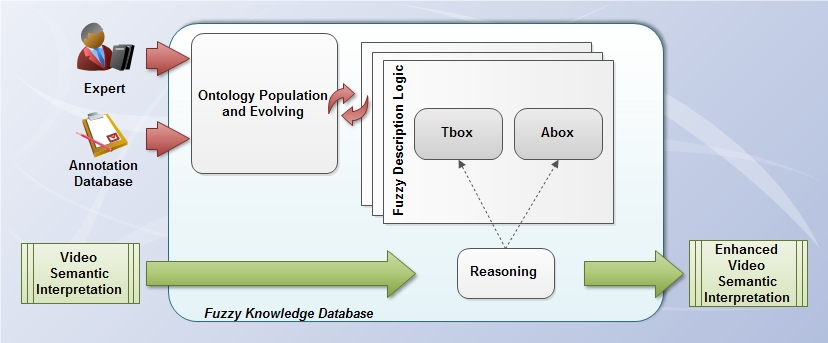
\includegraphics[width=\textwidth]{graphics/ontoSystem_2}
			\caption{The proposed multi fuzzy context-based ontology indexing 
						model for enhancing video semantic Interpretation}
			\label{fig:proposed_system}
		\end{figure}	

		\section{Ontology structure and population}

		\subsection{Knowledge representation}
		The purpose of constructing our ontologies is to model possible 
		relationships between semantic interpretations (concepts) within a defined context.
		Each ontology is considered as a knowledge database.
		Let $\mathcal{K}^{f}$ and $\mathbb{X}$ be respectively a set of fuzzy
		ontologies and a set of contexts defined as follow: 
		\begin{equation*}
			\begin{array}{ c c l }
			\mathbb{X} & = & \{t_{1}, t_{2}, \ldots, t_{n} \} \text{ a set of $n$ contexts,}\\
			\mathcal{K}^{f} & = &  \{\mathcal{K}^{f}_{t_{1}},\mathcal{K}^{f}_{t_{2}}, 
				\ldots, \mathcal{K}^{f}_{t_{n}}\} \text{ a set of $n$ fuzzy ontologies }  \\
				& &  \text{ where } \mathcal{K}^{f}_{t_{k}} \text{ is a fuzzy ontology for the context } t_{k}.
			\end{array}
		\end{equation*}
		
		And let $N_{C}$ be a set of concept names ($A$), $N_{R}$ a set of role names ($R$) 	
		and $N_{I}$ a set of individual names ($a$). 

		We use the three alphabets symbols for individuals, concepts and roles. Fuzzy knowledge axioms 
		are grouped in three parts: fuzzy $ABox$ $\mathcal{A}$ for individuals, fuzzy $TBox$ 
		$\mathcal{T}$ for concepts, and fuzzy $RBox$ $\mathcal{R}$ for roles. 

		\begin{definition}
		Formally, the ontology $\mathcal{K}^{f}_{t_{k}}$ 
		of the context $t_{k}$	
		can be defined as follows: 

		$\mathcal{K}^{f}_{t_{k}} = \langle \mathcal{T}, \mathcal{R}, \mathcal{A} \rangle$, where
		{
			\begin{equation*}
			\begin{array}{ c c l }
			\mathcal{T}  	& = 	& \{\mathsf{Shot} \sqsubseteq \top,\\
			&	& \mathsf{Concept} \sqsubseteq \top,\\
			&	& \mathsf{Context} \sqsubseteq \top,\\
			&	& \mathsf{Context}\sqsubseteq\leq{}1\mathsf{ExistsIn.Shot},\\
			&	& \mathsf{Shot}\sqsubseteq\exists\mathsf{indexedBy.Concept},\\
			&	& \mathsf{Concept} \sqsubseteq \exists{}\mathsf{isRelatedTo.Concept}\},\\
			\mathcal{A}	& = 	&
			\{(\langle{}\mathsf{Context},\mathsf{Shot}\rangle:\mathsf{ExistsIn})\geq
			p_{1}\\
			&	& (\langle{}\mathsf{Shot},\mathsf{Concept}\rangle:\mathsf{IndexedBy}) \geq	p_{2}\\
			&	& (\langle{}\mathsf{Concept},\mathsf{Concept}\rangle:\mathsf{isRelatedTo})
			\geq p_{3}\},\\
			\mathcal{R} 	& =	& \{\mathsf{Trans(isRelatedTo)} \\
			&	& \mathsf{Disjoint(isRelatedTo,isRelatedTo^{-})}\}
			\end{array}
		\end{equation*}
		}
		\end{definition}
		
		
		The shot is a temporal segment of a video. In our work, we detect
		shots through the segmentation approach provided by \emph{Christian Petersohn} 
		at the \emph{Fraunhofer Institute} \cite{Petersohn2004}. 
		Then, we extract one representative key-frame for each defined shot.
		
		The $TBox$ $\mathcal{T}$ contains intentional knowledge by describing general properties of concepts: 
		for the $\mathcal{K}^{f}_{t_{k}}$ structure, 
		we define the concepts $\mathsf{Shot}$, $\mathsf{Context}$ and $\mathsf{Concept}$. Then, we define three roles 
		$\mathsf{isRelatedTo(Concept,Concept)}$, $\mathsf{IndexedBy(Shot,Concept)}$ and $\mathsf{ExistsIn(Context,Shot)}$.
		
		
		
		The $TBox$  is usually thought not to change. This ontology structure is used for all context 
		based ontologies defined in this paper. However, 
		the $ABox$ $\mathcal{A}$ contains  extensional knowledge (assertional
		knowledge) which defines  individuals of a specific ontology. 
		Indeed, the $ABox$ $\mathcal{A}$ illustrates possible relationships 
		between concepts, contexts and video shots defined in the $TBox$ $\mathcal{T}$. 
		We would remind that the proposed ontology should support two knowledge
		kinds (see figure {\ref{fig:proposed_system}}): At first, a general knowledge
		is presented by the role $\mathsf{isRelatedTo(Concept, Concept)}$ which defines a generic semantic 
		relationship between two concepts. $p_{3}$ depicts the fuzzy weight of that 
		relationship. Then, the two roles $\mathsf{ExistsIn(Context, Shot)}$ and
		$\mathsf{IndexedBy(Shot, Concept)}$ are used for a particular 
		semantic interpretation of a given video shot. The role 
		$\mathsf{ExistsIn(Context, Shot)}$ depicts that the context 
		$\mathsf{Context}$ figures in the video shot $\mathsf{Shot}$ 
		with a fuzzy weight $p_{1}$. And the role $\mathsf{IndexedBy(Shot, Concept)}$ 
		depicts that the concept $\mathsf{Concept}$ exists in the video shot $\mathsf{Shot}$ 
		with a fuzzy weight $p_{2}$. These two roles represent both the initial 
		semantic interpretation and the enhanced one of a video shot.
		
		As an example, figure {\ref{fig:ontology_structure}} illustrates the ontology
		structure and individuals for the ontology $\mathcal{K}^{f}_{Indoor}$
		that is specific for the context $\mathsf{Indoor}$.
		} A video shot $\mathsf{Media1}$ is indexed by this context with a fuzzy
		degree of $0.8$. Then, the role $\mathsf{IndexedBy}$ $\mathsf{(Media1, Golf)}$
		depicts the fact that the video shot $\mathsf{Media1}$
		is indexed by the concept $\mathsf{Golf}$. And finally, 
		the role $\mathsf{isRelatedTo(Golf,News\_{}Strudio)}$ 
		defines a specific relationship between concepts $\mathsf{Golf}$ and $\mathsf{News\_{}Strudio}$ with a fuzzy 
		degree of $0.6$ within the ontology $\mathcal{K}^{f}_{Indoor}$. Thus, if a shot is relevant to the concept 
		$\mathsf{Golf}$, it could be relevant too to the concept $\mathsf{News\_{}Strudio}$ 
		if the context $\mathsf{Indoor}$ exists in this Shot.
		

		Any ontology based system developed by \emph{Description Logics} is able
		to perform specific kinds of reasoning. We discuss in what follows how we populate the ontologies,
		then, we describe the reasoning engine to enhance video semantic interpretation.
         
		\begin{figure*}[ht!]	
			\centering
			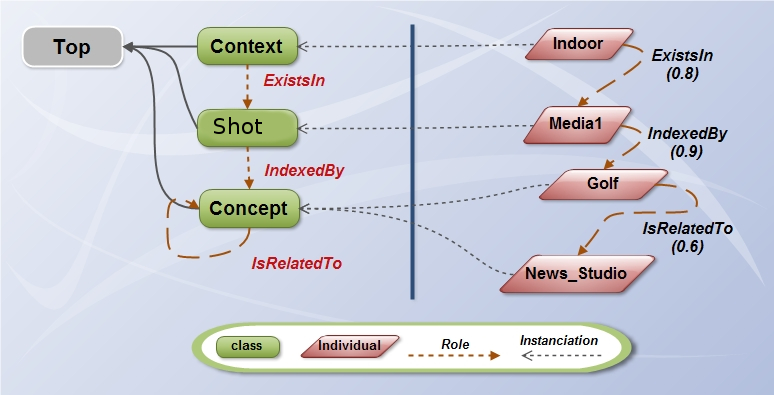
\includegraphics[width=\textwidth]{graphics/OntologyStructure_2}
			\caption{Fuzzy Knowledge Based Semantic Structure and Content 
			(Sample content of the ontology $\mathcal{K}^{f}_{Indoor}$) }
			\label{fig:ontology_structure}
		\end{figure*}

		\subsection{Ontology Populating}
		Our aim is to populate the ontology with new instances defined in a specific context, 
		as well as with their properties and relations. The initial ontology content is created by exploring 
		similarities between annotated video shots. The key idea behind our approach is that we can construct 
		relevant ontology content through a large video annotation database. 	
		In our work, we are particularly interested in the 
		\emph{ImageCLEF2012's Flickr Photo Annotation and Retrieval} \cite{Thomee2012} annotated 
		database to populate our ontologies. 

		%Therefore, a validation process is performed for improving the ontology content, and then the indexing 
		%effectiveness. In this section we point out steps for populating our set of ontologies.
		%\paragraph{Semantic Annotation}
		%	The aim of this stage is to annotate a corpus of video shots with existing concept instances. 
		%	At this level, we don't focus on how the corpus is annotated, but we consider that every 
		%	shots is tagged by a set of semantic concepts. 
		%\paragraph{Similarity Function}

		In what follows, we detail how to discover new knowledge content (particularly instances of the role 
		$\mathsf{isRelatedTo}$). Two different procedures are proposed: the first detects  
		$\mathsf{isRelatedTo}$ relationships without any defined context (non-contextualized relationships). 
		Discovered knowledge will be used as the content of a non contextualized ontology. 
		The second  procedure detects $\mathsf{isRelatedTo}$ relationships within a defined context 
		(contextualized relationships). The discovered knowledge will then be used as the content of 
		a contextualized ontology. Generated ontologies will be used afterwards to infer new knowledge.
		

		\subsubsection{Non-contextualized Knowledge Discovery}
			At this stage, in the context of ontology population, we aim to identify 
			new ontological instances. 
			For this purpose, we use similarity measurement to extract fuzzy 
			relationships between different concepts. 
			At runtime, each semantic concept $c$ is represented by a vector $V_{c}$  described as follows: 
			$V_{c} =\{v^{shot_{1}}_{c},v^{shot_{2}}_{c}, \dots, v^{shot_{m}}_{c}\}$ 
			where $v^{shot_{i}}_{c} \in [0,1]$ 
			is the tagged value of the concept $c$ for the video shot $shot_{i}$ fixed
			by the semantic annotation stage.

			Then, we compute the similarity $sim(c,d) $ between the two concepts $c$ and $d$. 
			This similarity will be used as a fuzzy degree for the relationship that relates the concepts
			$c$ to the concept $d$ within the role $\mathsf{isRelatedTo}$. 
			We use the vector space model based method to compute the similarity between concepts.
			\begin{equation}
				sim(c,d) = cossim(c,d) = \frac{\vec{V_{c}} . 
				\vec{V_{d}}}{|V_{c}| . |V_{d}|}
			\end{equation}
			where for each concept $c$, a weighted vector $V_{c}$ can be constructed as
			$\vec{V_{c}}=\{v_{1},\dots, v_{m}\}$ where $v_{i}$ is the weight of the concept $c$ in the video 
			shot $shot_{i}$, and 
			\begin{equation}
				v_{i}= tf_{shot_{i},c}.idf_{c} = tf_{shot_{i},c}.log\frac{|S|}{|s_{c}|}
			\end{equation}
			where $tf_{shot_{i},c}$ is the frequency of the concept $c$ in the
			video shot $shot_{i}$, $|S|$ is the total number of shots and $|s_{c}|$ is 
			the number of shots tagged by the concept $c$.

			We would like to remind that two issues are considered for this stage. 
			The first one is related to the fact that the role $\mathsf{isRelatedTo}$ is non symmetric 
			(as appears in the \emph{Rbox} $\mathcal{R}$). 
			As an example, when talking about the concept \emph{``car\_racing''}, 
			it is obvious that we talk about the concept \emph{``car''}, but  the opposit 
			in not often true. Thus $sim(car,car\_racing) \neq sim(car\_racing ,car)$.
			To do that, the similarity function that is used to compute the similarity $sim(c,d)$ has
			to be non symmetric. 
			Then, the two vectors $V_{c}$ and $V_{d}$ are modified as follow to ensure that  
			$sim(c,d) \neq sim(d,c)$:
			\begin{equation}
			\label{eq3}
			\begin{array}{ c c l }
			V_{c} & = & \{v^{shot_{1}}_{c},v^{shot_{2}}_{c}, \dots, v^{shot_{m'}}_{c}\}\\
			V_{d} & = & \{v^{shot_{1}}_{d},v^{shot_{2}}_{d}, \dots, v^{shot_{m'}}_{d}\}\\
			& & \text{where for every considered shot } shot_{i} \text{ in both } V_{c} \text{ and } V_{d},\\
			& & \text{we have } v^{shot_{i}}_{c}\neq 0.\\
			& & \text{And } m \geq m'. 
			\end{array}
			\end{equation}
			Only tagged shots by the concept $c$ are considered for both $V_{c}$ 
			and $V_{d}$ in order to guarantee the non symmetric aspect of the role $\mathsf{isRelatedTo}$.
			Accordingly, the size of the vectors $V_{c}$ and $V_{d}$ in equation
			\ref{eq3} ($m'$) is less or equal to the original size ($m$).
			
			The second issue deals with the context oriented proposed knowledge content. 
			In fact, the similarity measurement discussed above computes
			potential relationships degree between 
			two concepts without taking into account any defined context. 
			In this case, the extracted relationships 
			computed and extracted as shown above will be prepared to be inserted in a special non-contextualized 
			ontology. This latter does not contain any $\mathsf{Context}$ instance.
		
		\subsubsection{Contextualized Knowledge Discovery}
		This stage aims to discover relationships between concepts within a defined context.
		We would like to remind that a \emph{semantic context} is an abstract meaning that cannot be well defined because 
		it makes sense only in particular situations \cite{Elleuch2011, Ksentini2012}. 
		%%%%%%%%%%%%%%%%%%%%%%%%%%%%%%%%%%%%%%%%%%%%%%%%%%%%%%%%%%%%%%%%%%%%%%%%%%%%%%%%%%%%%%
		%%%%%%%%%%%%%%%%%%%%%%%%%%%%%%%%%%%%%%%%%%%%%%%%%%%%%%%%%%%%%%%%%%%%%%%%%%%%%%%%%%%%%%
		%%%%%%%%%%%%%%%%%%%%%%%%%%%%%%%%%%%%%%%%%%%%%%%%%%%%%%%%%%%%%%%%%%%%%%%%%%%%%%%%%%%%%%
		For example, the concept \emph{``airplane\_{}flying''} is considered as
		a context since it specifies a particular relationship between two other
		concepts: \emph{``sky'''} and \emph{``airplane''}. 
		%%%%%%%%%%%%%%%%%%%%%%%%%%%%%%%%%%%%%%%%%%%%%%%%%%%%%%%%%%%%%%%%%%%%%%%%%%%%%%%%%%%%%%
		%%%%%%%%%%%%%%%%%%%%%%%%%%%%%%%%%%%%%%%%%%%%%%%%%%%%%%%%%%%%%%%%%%%%%%%%%%%%%%%%%%%%%%
		%%%%%%%%%%%%%%%%%%%%%%%%%%%%%%%%%%%%%%%%%%%%%%%%%%%%%%%%%%%%%%%%%%%%%%%%%%%%%%%%%%%%%%
		In this paper, we define a context as follows:
		\begin{definition}
			A context is defined as a concept that can stipulate a specific relationship 
			between other concepts.
		\end{definition}
		Thanks to such a definition, we can give a more abstract meaning of a context
		rather than a spatial or temporal information \cite{Brilhault2009},
		and also provide an automated way to discover contexts within a concept set.
		
		Then, for a given concept $c$, we look for some eventual relationships
		between other concepts within shots annotated with the concept $c$. 
		If such relationships are found, the concept $c$ is considered as a context.

		Based on what has just been developed, we propose a formal method to discover contexts. 
		In our case, we populate a fuzzy ontology $\mathcal{K}^{f}_{t_{k}}$ of the context $t_{k}$ as follows:
		%%%%%%%%%%%%%%%%%%%%%%%%%%%%%%%%%%%%%%%%%%%%%%%%%%%%%%%%%%%%%%%%%%%%%%%%%%%%%%%%%%%%%%
		%%%%%%%%%%%%%%%%%%%%%%%%%%%%%%%%%%%%%%%%%%%%%%%%%%%%%%%%%%%%%%%%%%%%%%%%%%%%%%%%%%%%%%
		%%%%%%%%%%%%%%%%%%%%%%%%%%%%%%%%%%%%%%%%%%%%%%%%%%%%%%%%%%%%%%%%%%%%%%%%%%%%%%%%%%%%%%			
		We define the similarity $sim_{t_{k}}(c, d)$ as a similarity measurement between the 
		two concepts 
		$c$ and $d$ within the context $t_{k}$. This similarity will be used as fuzzy degree 
		for the rule that relates the concepts $c$ to the concept $d$ within the role 
		$\mathsf{isRelatedTo}$ for the $\mathcal{K}^{f}_{t_{k}}$ ontology.

		Considering the non symmetric aspect of the role $\mathsf{isRelatedTo}$ discussed in the previous section, 
		vectors $V_{c}$ and $V_{d}$ used to compute $sim_{t_{k}}(c, d)$ are defined as follows:
		%%%%%%%%%%%%%%%%%%%%%%%%%%%%%%%%%%%%%%%%%%%%%%%%%%%%%%%%%%%%%%%%%%%%%%%%%%%%%%%%%%%%%%
		%%%%%%%%%%%%%%%%%%%%%%%%%%%%%%%%%%%%%%%%%%%%%%%%%%%%%%%%%%%%%%%%%%%%%%%%%%%%%%%%%%%%%%
		%%%%%%%%%%%%%%%%%%%%%%%%%%%%%%%%%%%%%%%%%%%%%%%%%%%%%%%%%%%%%%%%%%%%%%%%%%%%%%%%%%%%%%		
		
		\begin{equation}
			\label{eq4}
			\begin{array}{ c c l }
			V_{c} & = & \{v^{shot_{1}}_{c},v^{shot_{2}}_{c}, \dots,
			v^{shot_{m''}}_{c}\}\\
			%%%%%%%%%%%%%%%%%%%%%%%%%%%%%%%%%%%%%%%%%%%%%%%%%%%%%%%%%%%%%%%%%%%%%%%%%%%%%%%%%%%%%%
			%%%%%%%%%%%%%%%%%%%%%%%%%%%%%%%%%%%%%%%%%%%%%%%%%%%%%%%%%%%%%%%%%%%%%%%%%%%%%%%%%%%%%%
			%%%%%%%%%%%%%%%%%%%%%%%%%%%%%%%%%%%%%%%%%%%%%%%%%%%%%%%%%%%%%%%%%%%%%%%%%%%%%%%%%%%%%%			
			%V_{d} & = & 
			V_{d} & = & 
			%%%%%%%%%%%%%%%%%%%%%%%%%%%%%%%%%%%%%%%%%%%%%%%%%%%%%%%%%%%%%%%%%%%%%%%%%%%%%%%%%%%%%%
			%%%%%%%%%%%%%%%%%%%%%%%%%%%%%%%%%%%%%%%%%%%%%%%%%%%%%%%%%%%%%%%%%%%%%%%%%%%%%%%%%%%%%%
			%%%%%%%%%%%%%%%%%%%%%%%%%%%%%%%%%%%%%%%%%%%%%%%%%%%%%%%%%%%%%%%%%%%%%%%%%%%%%%%%%%%%%%			
			\{v^{shot_{1}}_{d},v^{shot_{2}}_{d}, \dots, v^{shot_{m''}}_{d}\}\\
			& & \text{ where for every considered shot } shot_{i} \text{ in both } V_{c} \text{ and } V_{d},\\
			& &  \text{we have } v^{shot_{i}}_{c}\neq 0 \text{ and } v^{shot_{i}}_{t_{k}}
			\geqslant \gamma.\\
			& & \text{And } m \geq m' \geq m''.
			\end{array}
		\end{equation}
		we suggest $\gamma \in [0,1]$  as a threshold to judge if a concept is strongly relevant 
		to a video shot or not. Thus, only tagged shots by the concept $c$ and that are strongly 
		tagged by the concept/context $t_{k}$ are considered for both $V_{c}$ and $V_{d}$ in order to guarantee 
		the non symmetric aspect of the role $\mathsf{isRelatedTo}$.
		
		\subsection{Pattern-based ontology Content manager}
		
		\begin{figure}[ht!]	
		\begin{center}
			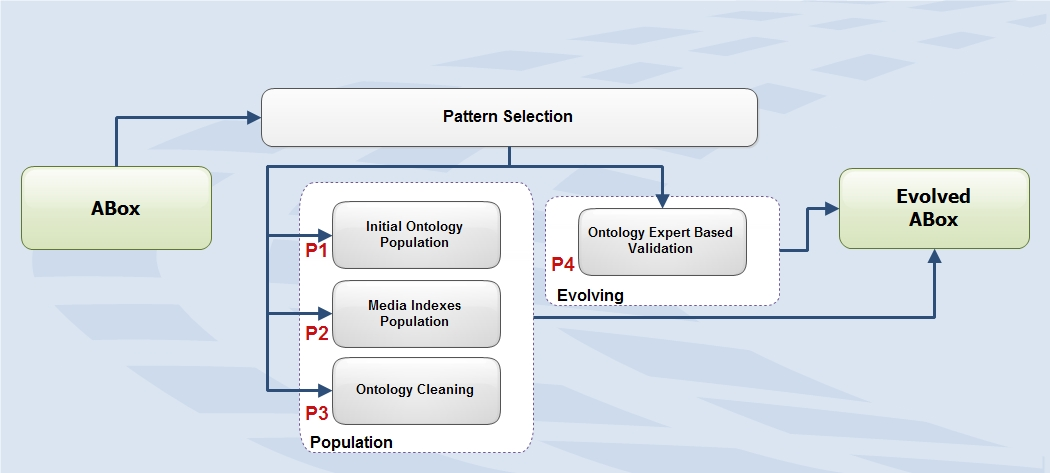
\includegraphics[width=\textwidth]{graphics/patterns_2}
			\caption{Four Patterns for ontology content manager}
			\label{fig:patterns}
		\end{center}
		\end{figure}
		
		In order to manage ontology contents, we propose the use of four different patterns. 
		Three different cases have been identified for the population task, and only one pattern is identified 
		for the evolving task (see figure \ref{fig:patterns}). We underline that these patterns deal with the 
		$Abox$ $\mathcal{A}$ part of the ontologies, and the $Tbox$ $\mathcal{T}$ remains unchanged.
		
		The pattern $P1$ is called by the population process when new $\mathsf{isRelatedTo}$ 
		roles are defined for a specific context. Then we create a separate ontology for every context, 
		the context itself is introduced in the ontology (as an individual of the class $\mathsf{Context}$). 
		After that, the defined concepts for this context are introduced 
		(as individuals of the class $\mathsf{Concept}$). 
		Finally, the discovered roles within the specific context are inserted in the ontology (as instantiation of
		the role $\mathsf{isRelatedTo}$). 

		The pattern $P2$ is used to add the initial indexes of a given video shot to an ontology.
		Then, this shot is added to all the defined ontologies (as an individual of
		the class $\mathsf{Shot}$).
		Then, for every ontology, we instantiate the two roles $\mathsf{ExistsIn}$ between the given 
		context for this ontology and the shot, and $\mathsf{IndexedBy}$ between the shot and tagged concepts.
		
		
		We underline that the pattern $P2$ is used for a given video shot. And to handle another new video 
		shot, we have to remove all data except the $\mathsf{Context}$/$\mathsf{Concept}$ individuals and 
		$\mathsf{isRelatedTo}$ role instantiations. This cleaning task is done by the pattern $P3$.

		Finally, we define one evolution pattern $P4$ for the ontology evolution. 
		This pattern consists of a set of activities to be performed on an $Abox ~ \mathcal{A}$
		to apply all the required updating changes. The evolution pattern 
		$P4$ describes the situation where a new $\mathsf{isRelatedTo}$ role fuzzy weight is defined.
	
		\section{Reasoning with Ontologies to enhance Semantic Interpretation}

		The defined set of fuzzy context-based ontologies are used to enhance video semantic 
		interpretation through a fuzzy reasoning process. Within the scope 
		of reasoning in this paper, we are particularly interested in the outputs that
		such a system produces. In addition to initial ontologies content (particularly concepts/contexts and 
		$\mathsf{isRelatedTo}$ roles), we add some new contents for each analyzed video. Indeed, videos are 
		generally segmented to shots, and every shot is interpreted by a set of concepts.
		Then, and for each ontology $\mathcal{K}^{f}_{t_{k}}$ of a context $t_{k}$, we generate 
		the corresponding ontology $\mathcal{K'}^{f}_{t_{k}}$ as a content enhancement. This is done by 
		interpreting the $Abox$ $\mathcal{A}$ in order to look for updated or additional relationships between 
		$\mathsf{Shot}$ and $\mathsf{Concept}$ (for the role name
		$\mathsf{isIndexedBy}$).

		In this paper, we used and adapted a \emph{``tableau''} based reasoning algorithm \cite{Dentler2011}. This algorithm 
		adopts a federated reasoning process with our set of fuzzy ontologies. Thus, each fuzzy ontology is 
		associated with a local reasoner. The final and global reasoning  result is inferred through 
		all the local reasoner results. 


		Considering concepts and roles as fuzzy sets, the semantics of concepts and roles are defined 
		by fuzzy interpretations $\mathcal{I} = \langle{}\triangle^{\mathcal{I}}= , \cdot^{\mathcal{I}}\rangle{}$, 
		where $\triangle^{\mathcal{I}}$ is a nonempty domain, and $\cdot^{\mathcal{I}}$ is an interpretation 
		function mapping individuals $a$ into $a^{\mathcal{I}} \in \triangle^{\mathcal{I}}$,
		and mapping concept (roles) names $A(R)$ into membership functions 
		$A^{\mathcal{I}}(R^{\mathcal{I}}) : \triangle^{\mathcal{I}} (\triangle^{\mathcal{I}} × \triangle^{\mathcal{I}} ) 
		\rightarrow [0, 1]$. 
		An interpretation $\mathcal{I}$ satisfies a knowledge database $\mathcal{K}^{f}_{}$, 
		if and only if  $\mathcal{I}$ satisfies any
		axiom in $\mathcal{R}$, $\mathcal{T}$ and $\mathcal{A}$. $\mathcal{K}^{f}_{}$ is satisfiable 
		if and only if it has a fuzzy model.

		We define the symbols  $\rhd$ and  $\lhd$ as a placeholder for the  inequalities 
		($\leq$, $<$, $\geq$ and $>$) and the symbol $\bowtie$ as a placeholder for all types of inequalities.
		
		\begin{definition}
			let $R_{A}$ be the set of roles occurring in $\mathcal{A}$, $I_{\mathcal{A}}$ the set 
			of individuals in $\mathcal{A}$ and $\mathcal{X} = \{\leq, <, \geq, >\}$. A fuzzy tableau 
			$T$ for $\mathcal{A} ~ w.r.t ~ \mathcal{R}$ is a quadruple
			$(S, \mathcal{L, E, V})$ in such a way that:
			\begin{itemize}
				\item $S$ is a nonempty set of individuals (considered also as nodes),
				\item $\mathcal{L} : S \longrightarrow 2^{sub(A)} \times \mathcal{X} \times [0,1]$ 
					maps each individual in $S$ to membership triples,
				\item $\mathcal{E} : R_{A} \longrightarrow 2^{S \times S} \times \mathcal{X} \times [0,1]$ 
					maps each role to membership triples,
				\item $\mathcal{V} : I_{\mathcal{A}} \longrightarrow S$ maps individuals occurring in 
					$\mathcal{A}$ to elements in $S$.
			\end{itemize}
		For all	$s,t \in S$, $R\in R_ {A}$ and $C,E \in sub(\mathcal{A})$, $T$ satisfies a particular 
		transformation rule defined in algorithms \ref{algo1} and \ref{algo2}
		(in addition to default transformation rules defined in \cite{Stoilos2005}).	

		\begin{algorithm}
				\label{algo1}
				\If	{ $\langle(t_{k},shot_{i}) : \mathsf{ExistsIn} \bowtie \alpha_{1}\rangle 
					\in \mathcal{A}$ AND \\
					$\langle(shot_{i},c) : \mathsf{IndexedBy} \bowtie \alpha_{2}\rangle \in \mathcal{A}$ 
					AND \\
					$\langle(c,d) : \mathsf{isRelatedTo} \bowtie \alpha_{3}\rangle \in \mathcal{A}$}
					{
					 \lIf	{$\langle(shot_{i},d) : \mathsf{IndexedBy} \bowtie 
						\alpha_{4}\rangle \notin \mathcal{A}$} 
						{\\$\mathcal{A'} := \mathcal{A} \sqcup \{ \langle{}\mathsf{shot_{i}},
							\mathsf{d}\rangle:
							\mathsf{IndexedBy}) \bowtie \alpha_{4}\}$\\
							and $\langle \langle\mathcal{V}(shot_{i}),\mathcal{V}(d)\rangle
							\bowtie \alpha_{4}\rangle 
							\in \mathcal{E}(\mathsf{IndexedBy})$ \\
							where $\alpha_{4} = \alpha_{1} \times \alpha_{2} \times \alpha_{3}$}
						\lElse{$\langle \langle\mathcal{V}(shot_{i}),\mathcal{V}(d)\rangle
							\bowtie \alpha_{4}'\rangle 
							\in \mathcal{E}(\mathsf{IndexedBy})$ \\
							where $\alpha_{4}' = max(\alpha_{4}, (\alpha_{1} \times \alpha_{2}
							\times \alpha_{3}))$}
					}
					\caption{Transformation Rule: Property 1}
				\end{algorithm}
				\begin{algorithm}
				\label{algo2}
				\If	{ $\langle(t_{k},shot_{i}) : \mathsf{ExistsIn} \bowtie \alpha_{1}\rangle 
					\notin \mathcal{A}$ AND \\
					$\langle(shot_{i},c) : \mathsf{IndexedBy} \bowtie \alpha_{2}\rangle 
					\in \mathcal{A}$ AND \\
					$\langle(c,d) : \mathsf{isRelatedTo} \bowtie \alpha_{3}\rangle \in \mathcal{A}$}
					{
					 \lIf	{$\langle(shot_{i},d) : \mathsf{IndexedBy} \bowtie \alpha_{4}\rangle
						\notin \mathcal{A}$}
						{\\$\mathcal{A'} := \mathcal{A} \sqcup \{ \langle{}\mathsf{shot_{i}},
							\mathsf{d}\rangle:
							\mathsf{IndexedBy}) \geq \alpha_{4}\}$\\
							and $\langle \langle\mathcal{V}(b),\mathcal{V}(d)\rangle
							\bowtie \alpha_{4}\rangle 
							\in \mathcal{E}(\mathsf{IndexedBy})$ \\
							where $\alpha_{4} = \alpha_{2} \times \alpha_{3}$}
						\lElse{$\langle \langle\mathcal{V}(shot_{i}),\mathcal{V}(d)\rangle
							\bowtie \alpha_{4}'\rangle 
							\in \mathcal{E}(\mathsf{IndexedBy})$ \\
							where $\alpha_{4}' = max(\alpha_{4}, (\alpha_{2} \times \alpha_{3}))$}
					}
					\caption{Transformation Rule: Property 2}
				\end{algorithm}
		\end{definition}
		Property 1 is a consequence of the fact that if there are three
		axioms in $\mathcal{A}$ where $shot_{i}$ is indexed by a 
		concept $c$, and the context $t_{k}$ exists in the $shot_{i}$, 
		then the $shot_{i}$ could be indexed by the concept $d$ taking into account that within the 
		fuzzy ontology of the context $t_{k}$, there is a relationship between the two concepts $c$ and $d$.
		If this new deduced relationship exists in the ontology, then we only update its fuzzy weight.
		
		Property 2 proceeds in the same way as the first. However, it deals with 
		a non-contextualized ontology (the role $\mathsf{ExistsIn}$ does not exists in $Abox$ $\mathcal{A}$).
		
		We used and adapted a \emph{“tableau”} based reasoning algorithm.
For a given context-based ontology, the latter model the knowledge in form of 
a tree in which nodes correspond to individuals (semantic concepts, semantic context and shots) 
and edges correspond to roles ($\mathsf{isIndexedBy}$,$\mathsf{isRelatedTo}$,
and $\mathsf{ExistsIn}$).
Each node $x$ is labeled with a set of concepts $\mathsf{L}(x)$ that the
individual must satisfy, and each edge is labeled with a role name.
The reasoning algorithm starts with a single node labeled $\{D\}$ (in our cas, a
node labeled as a shot), and proceeds by repeatedly applying a set of expansion 
rules that recursively decompose the concepts in node labels.

The reasoning process should 
always terminate. But proving the termination is hard for cases where the ontology includes 
transitive roles (like the $\mathsf{isRelatedTo}$ role). This problem can dealt with the use 
of a blocking technique: stopping the expansion when a cycle is detected. The blocking 
procedure consists in checking the label of each new node $y$, and if it's a subset of the 
label of an existing node $x$, then the expansion of $y$ is stopped: $x$ is said to block $y$.
 The reasoning process termination is guarantied: all concepts in node labels are derived 
 from the decomposition of $D$, so all node labels must be a subset of the sub-concepts of $D$. 
A cycle should be avoided within a finite number of expansion steps.


%%%%%%%%%%%%%%%%%%%%%%%%%%%%%%%%%%%%%%%%%%%%%%%%%%%%%%%%%%%%%%%%%%%%%%%%%%%%%%%%%%%%%%%%%%%%%%%%%%
%%%%%%%%%%%%%%%%%%%%%%%%%%%%%%%%%%%%%%%%%%%%%%%%%%%%%%%%%%%%%%%%%%%%%%%%%%%%%%%%%%%%%%%%%%%%%%%%%%
\begin{algorithm}
			\label{algo112}
			\SetAlgoLined
			%\KwData{$Input \neq \emptyset$ and $Output = \emptyset$ }
			%\KwResult{$Output \neq \emptyset$ }
			\For{each shot \textbf{$shot_{i} \in \mathsf{Shot}$}}{
				\For{each concept \textbf{$c$} connected with the shot 
				\textbf{$shot_{i}$} by an $\mathsf{isIndexedBy}$ labeled edge}{
					Handle\_isRelatedTo\_Role($shot_{i}$,$c$);
				}
			}
			\caption{Reasoning Process for enhancing a semantic interpretation about
			shots.}
		\end{algorithm}
		
%%%%%%%%%%%%%%%%%%%%%%%%%%%%%%%%%%%%%%%%%%%%%%%%%%%%%%%%%%%%%%%%%%%%%%%%%%%%%%%%%%%%%%%%%%%%%%%%%%
%%%%%%%%%%%%%%%%%%%%%%%%%%%%%%%%%%%%%%%%%%%%%%%%%%%%%%%%%%%%%%%%%%%%%%%%%%%%%%%%%%%%%%%%%%%%%%%%%%
		
		\begin{algorithm}
			\label{algo111}
			\SetAlgoLined
			%\KwData{$Input \neq \emptyset$ and $Output = \emptyset$ }
			%\KwResult{$Output \neq \emptyset$ }
			\textbf{Function} Handle\_isRelatedTo\_Role($shot_{i}$,$c$)\\
			  \eIf{isMarked($c$)}{
			  return\;}
			  {
			  		\For{each concept $d$ connected with $c$ by an edge labeled
			  		$\mathsf{isRelatedTo}$}{Mark($c$)\;
					apply Algorithms \ref{algo1} and \ref{algo2}\;
					Handle\_isRelatedTo\_Role($shot_{i}$,$d$)\;
				}	
			}
			\caption{Recursive call for \emph{``Handle\_isRelatedTo\_Role()''} Function}
		\end{algorithm}
%%%%%%%%%%%%%%%%%%%%%%%%%%%%%%%%%%%%%%%%%%%%%%%%%%%%%%%%%%%%%%%%%%%%%%%%%%%%%%%%%%%%%%%%%%%%%%%%%%
%%%%%%%%%%%%%%%%%%%%%%%%%%%%%%%%%%%%%%%%%%%%%%%%%%%%%%%%%%%%%%%%%%%%%%%%%%%%%%%%%%%%%%%%%%%%%%%%%%

The defined $\mathsf{isRelatedTo}$ role is cyclic and transitive. Such a
definition make the  termination and the decidability of our reasoning process hard. We adapted 
the \emph{``tableau''} algorithm is such a way to  solve this problem. 
Apart from the generic blocking technique above detailed, we used a second 
blocking technique which marks every passage through  
semantic concepts that are connected with $\mathsf{isRelatedTo}$ role labeled
edges. We used two functions: $Mark(c)$ which marks a concept $c$, and
$isMark(c)$ which returns whether the concept $c$ is marked or not yet.

Algorithms \ref{algo112} and \ref{algo111} detail how we extend a semantic interpretation of a given
shot taking into consideration the proposed blocking technique. 

The node marking test in the algorithm \ref{algo111} allows to detect an
eventual cycle. Then, a possible endless call to the
\emph{``Handle\_isRelatedTo\_Role()''} recursive function is blocked. 
The proposed algorithm achieved the decidability of our reasoning process.

  


		\section{Ontology Evolving}
		\label{section:evolving}
		The ontology evolution is a crucial task that must be addressed in an ontology life cycle. 
		It consists in updating the ontology content in order to take into account eventual erroneous 
		or senseless knowledge. In our work, we consider the evolution of ontology individuals content 
		and not the conceptual level. Then, only individuals and inter-relationships in $Abox$ $\mathcal{A}$ 
		could be updated. The pattern $P4$ for ontology evolving is used for such a case.
	
		Let $\mathcal{A}$ be the $ABox$ of an ontology, and $\mathcal{A_{+}}$ 
		the updated $ABox$. %, and $\mathcal{A'}$ the final considered knowledge after
		% the evolving process.
		 Then the evolution pattern $P4$ activities can be illustrated with the
		algorithm \ref{algo3}.
		
		\begin{algorithm}
				\label{algo3}
				\If	{$\langle(c,d) : \mathsf{isRelatedTo} \bowtie \alpha \rangle \in \mathcal{A}$ AND \\
					 $\langle(c,d) : \mathsf{isRelatedTo} \bowtie \alpha'\rangle \in \mathcal{A_{+}}$ }
					{
					 $\mathcal{A} := \mathcal{A}  \diagdown \{
					 \langle{}(\mathsf{c},\mathsf{d}):
							\mathsf{isRelatedTo}\rangle{} \bowtie \alpha\}$\\
					$\mathcal{A} := \mathcal{A} \sqcup \{ \langle{}(\mathsf{c},\mathsf{d}):
							\mathsf{isRelatedTo}\rangle{} \bowtie \alpha'\}$\\
					}
				\caption{The evolving pattern $P4$}
		\end{algorithm}

		We outline that the pattern evolution $P4$ always takes the new discovered knowledge by 
		updating the fuzzy weight of a $\mathsf{isRelatedTo}$ role to 
		the new value defined in $\mathcal{A_{+}}$.

		Let's now show how we generate the new $ABox$ $\mathcal{A_{+}}$ used to update the ontology content. 
		In our work, we consider that the set of ontologies are populated through
		a knowledge discovery based 
		on video annotation data. We consider, too, that this extracted knowledge may
		be erroneous depending on some factors (annotators, video database quality, \dots). 
		We propose  to correct ontologies content 
		through inspecting $\mathsf{isRelatedTo}$ roles by human experts. 
		We thus propose a user interface where experts give their judgment on the relevance of a role in a
		particular context.

		For a particular context $t_{k}$ and an affiliated $\{ \langle{}(\mathsf{c},\mathsf{d}): 
		\mathsf{isRelatedTo}\rangle{} \bowtie \alpha\}$ role, this user interface shows
		the expert a set of rows where each one details one shot that both the context 
		$t_{k}$ and the concept $c$ exist. The expert then has to select one from these four options:
		\begin{itemize}
			\item $Strongly~Relevent$ when the concept $d$ effectively in the showed shot. We 
				consider that the fuzzy weight for this case is higher or equal to $0.7$,
			\item $Weakly~Relevent$ When the concept $d$ may exists in the showed shot. We 
				consider that the fuzzy weight for this case is higher or equal to $0.3$ 
				and lower than $0.7$,
			\item $Not~Relevent$ When the concept $d$ does not exist in the showed shot. We 
				consider that the fuzzy weight for this case is lower than $0.3$,
			\item $Skip$ when the expert can not judge clearly if the concept $d$ 
				exists or not in the showed shot.
		\end{itemize} 
		
		The original value of a fuzzy weight of a given role is taken into
		consideration and appears when the evolving user interface displays a role to 
		an expert. In fact, every role is displayed 
		with its fuzzy weight, and the expert judge to input his judgment (if he
		founds that the role is not pertinent) or to skip to analyze another role.
		
		After the evaluation process done by the experts, the evolving pattern $P4$ computes new fuzzy 
		weights for evaluated roles. These weights are computed as follows:
		Let $N_{experts}$ be the number of experts who evaluated the role $r$. Let $N_{StrongR}$, 
		$N_{WeakR}$ and $N_{NotR}$ be, respectively, the number of $Strongly~Relevent$, $Weakly~Relevent$ 
		and $Not~Relevent$ judgments made by the $N_{experts}$ experts for the role $r$ where:
		\begin{equation}
			N_{experts} \geqslant  N_{StrongR} +  N_{WeakR} +  N_{NotR}.
		\end{equation}

		Then, we compute the new fuzzy weight for the evaluated role $r$ as follows:
		
		\begin{equation}
		\alpha'=\left\{
			\begin{array}{l c}
				max(\alpha, \frac{N_{StrongR}}{N_{experts}})	& 
					\text{\scriptsize{if $N_{StrongR} \geqslant (N_{WeakR},N_{NotR})$}} \\
				min(\alpha, \frac{1-N_{WeakR}}{N_{experts}}) & 
					\text{\scriptsize{if $N_{WeakR} > (N_{StrongR},N_{NotR})$}}\\
				min(\alpha, \frac{1-N_{NotR}}{N_{experts}})  &
					\text{\scriptsize{if $N_{NotR} > (N_{StrongR},N_{WeakR})$}}
			\end{array}
		  \right.
		\end{equation}

		The equation above is inspired by the majority vote. Indeed, the new computed role 
		fuzzy weight is based on whether experts are commonly improving or disregarding a role.
		
		For an analyzed role, only one new fuzzy weight will be considered
		and introduced to the ontology. Thus, no eventual conflicting situation 
		occurs when firing the reasoning engine.
		This choice is preselected by the initial value of fuzzy role weight.
	
		\section{Proposed Approach Scalability}
		The scalability of our approach is very important
		and concerns mainly two aspects: how does it perform when a large amount of concepts 
		and interrelationships are defined, and when the number of contexts
		increases. Our proposed approach can be considered as scalable:
		Firstly, the $Tbox$ $\mathcal{T}$ remains unchanged, and only new $Abox$ $\mathcal{A}$ 
		instances will be handled within the ontology. Then, the amount of knowledge 
		stored in an ontology depends only on what has been gathered from annotated 
		video datasets in addition to the semantic interpretation of the analyzed video shot. 
		Secondly, since the proposed approach is decomposed into several ontologies, 
		the deduction engine is applied only on
		$Abox$ $\mathcal{A}$ that are related only to each defined contexts. 
		This leads to an optimized and a lightened reasoning process: only partial 
		defined roles in ontologies will be considered and fired.
		
		In the next section, we conduct an experiment to investigate our
		approach effectiveness and scalability using a large video database.


\section{Conclusion}

In this chapter, we presented a fuzzy context-based ontology generation framework for enhancing a semantic interpretation about a multimedia content. The proposed framework deals with an abduction engine for extracting valuable knowledge (contexts, concepts and their relationships) from available data sources, and a deduction engine for inferring new knowledge from extracted ones. In the next chapter, we prouve our framework effectiveness and performance within diverse benchmarks (mainly \textsc{TrecVid2010} and \emph{ImageCLEF2012's Flickr Photo Annotation and Retrieval}).
